\documentclass{../../template/labo}

\usepackage[utf8x]{inputenc}
\usepackage[T1]{fontenc}
\usepackage{charter}
\usepackage{ucs}
\usepackage{amsthm} %numéroter les questions
\usepackage{amsmath}
\usepackage[frenchb]{babel}
\usepackage{datetime}
\usepackage{xspace} % typographie IN
\usepackage{hyperref}% hyperliens
\usepackage[all]{hypcap} %lien pointe en haut des figures
\usepackage[french]{varioref} %voir x p y
\usepackage{fancyhdr}% en têtes
\usepackage[]{graphicx} %include pictures
\usepackage{tikz}
\usetikzlibrary{babel,positioning,calc}
\usepackage[siunitx]{circuitikz}
\usepackage{mathastext} % math as standfard text : units are respecting typography conventions.
\usepackage{siunitx}
\usepackage{amssymb}
\usepackage{gnuplottex}
\usepackage{ifthen}
\usepackage{xcolor}
\usepackage{float}
%\usepackage{footmisc}
\usepackage[normalem]{ulem}

%\usepackage[top=1.3 in, bottom=1.3 in, left=1.3 in, right=1.3 in]{geometry} % Yeah, that's bad to play with margins
\usepackage[]{pdfpages}

\usepackage[]{attachfile}

%%%%%%%%%%%%
% Tables
%%%%%%%%%%%%
\usepackage{booktabs}
\renewcommand{\arraystretch}{1.1} % Opens up the table a tad
\usepackage{multicol}
\usepackage{multirow}

\langexam{frenchb}

\newboolean{koriG}
\ifx\koriG\undefined
\correction{false}
\else
\correction{true}
\fi

% \correction{false}
%\correction{true}

\author{The Fantastic Four} %<3

\pagestyle{fancy}
\lhead{[AE3T] Laboratoire d'électronique appliquée\\ Labo 3~: Transistor MOS\ifthenelse{\boolean{corrige}}{~-- corrigé}{}}
\rhead{v1.0.1\\ page \thepage}
\cfoot{}
%%



\setlength{\parindent}{0pt}

\begin{document}

\tptitle{}{Labo 3~: Réalisation d'un ampli à transistor}



% ########   ##      ##  ##########  ########     #####    
%    ##      ###     ##      ##      ##     ##  ##     ##  
%    ##      ## ##   ##      ##      ##     ##  ##     ##  
%    ##      ##  ##  ##      ##      ########   ##     ##  
%    ##      ##   ## ##      ##      ##   ##    ##     ##  
%    ##      ##     ###      ##      ##    ##   ##     ##  
% ########   ##      ##      ##      ##     ##    #####    

\section{Introduction}

Au cours de ce laboratoire, vous réaliserez un montage amplificateur à l'aide d'un transistor NMOS.
Vous aurez l'occasion de mettre votre montage à l'épreuve avec différents signaux en entrée et différentes résistances pour observer l'impact de la polarisation sur le comportement du transistor. Vous visualiserez aussi clairement les limites de fonctionnement de ce dernier.\\


À la fin de ce laboratoire, vous devez être capable :
\begin{itemize}
\item de réaliser l'amplificateur avec un étage source commune ;
\item d'expliquer le fonctionnement de l'étage source commune et sa polarisation ;
\item d'utiliser le mode XY d'un oscilloscope.
\end{itemize}

\subsection{Matériel}

\begin{center}
	\begin{tabular}{p{0.2\textwidth}rlp{0.1\textwidth}}
		Composant & \multicolumn{2}{c}{Valeur} & Quantité \\\toprule
		\multirow{5}{*}{Résistance} & 22 & $\Omega$ & x1 \\
									& 10 & $k\Omega$ & x1 \\
									& 22 & $k\Omega$ & x1 \\\midrule
		\multirow{1}{*}{Condensateur} 	& 10 & $\si{\nano\farad}$ & x2 \\\midrule
		Transistor & BS170 & & x1 \\\bottomrule
	\end{tabular}
	\end{center}
\clearpage

% ########   ##     ##  
%    ##      ##     ##  
%    ##      ##     ##  
%    ##      ##     ##  
%    ##       ##   ##   
%    ##        ## ##    
% ########      ###   
\section{Caractérisation du transistor}

Le transistor utilisé dans ce laboratoire est un BS170. Référez-vous à sa fiche technique lorsque des résultats analytiques sont demandés.

Avant de dimensionner l'étage en source commune, il est nécessaire de caractériser le transistor afin de déterminer sa transconductance $g_m$. % pour un point de fonctionnement donné.
On cherche en particulier à déterminer sous quelles conditions il se comporte comme une source de courant commandée en tension.

\subsection{Caractéristique $I_D=f(V_{GS})$}

Pour relever la caractéristique $I_D=f(V_{GS})$, vous utiliserez le montage suivant. La résistance $R_D$ sert à limiter le courant traversant le transistor pour ne pas le détruire.
\ctikzset{tripoles/mos style/arrows}
%\begin{figure}[H]
	\begin{center}
		\begin{circuitikz}[scale=0.8]%[american voltages]
		\draw
		(0,0) to [V=$e(t)$] (0,2)
		(0,2) to [short] (1,2)
		(0,0) to (1,0)
		(1,2) to [open, v^<=$V_{GS}$](1,0)
		(1,0) to [short, o-] (2,0)
		(3,2) node[nfet] (mos) {}
		(3,0) to [short] (mos.S)
		(1,2) to [short] (mos.G)
		(mos.B) -- (mos.S)
		(2,0) to (3,0)
		(mos.D) to [short, i<=$I_D$](3,3)
		(3,3) to [R,l=$R_D$ ] (3,5)
		%(3,3.2) to [short] (4,3.2)
		(3,5) to (4,5)
        %(4,3.2) node[esource] (voltm) {V}
		%(4,3.2) to (4,5)
		%(2,0) -- (5,0) to [battery, l_=$12V$] (5,5) -- (3,5)
		(2,0) -- (5,0)
		(5,5) -- (3,5)
		(5,5) to [battery, l=$E (5V)$] (5,0)
		(3,0) node[ground] {}
		;\end{circuitikz}
	\end{center}
	\vspace*{-0.5cm}
%\caption{Montage pour relever $I_D=f(V_{GS})$}
%\label{fig:scidvgs}
%\end{figure}

\Question{\label{Q:det_rd}
Quelle est la puissance maximale que le transistor peut dissiper ?
Déterminez $R_D$ tel que le transistor ne dépasse pas cette puissance. 

\begin{astuce}
	Trouvez d'abord l'expression de la puissance dissipée par le transistor en fonction de son courant de drain $I_D$. Trouvez ensuite la valeur de $I_D$ maximisant la puissance.
\end{astuce}
}
{

La datasheet nous indique que la puissance maximale que le transistor peut dissiper est de 830~mW.

$P_T$ est la puissance dissipée par le \textbf{transistor} et $E$ la tension d'alimentation connectée à $R_D$.

$$P_T=V_{DS}\cdot I_D = \left(E-R_D\cdot I_D \right)\cdot I_D$$
d'où : $$ P_T=E\cdot I_D - R_D \cdot {I_D}^2$$

L'extremum (ici : maximum) se trouve en :

$$\frac{\partial P_T}{\partial I_D}=0 \Longleftrightarrow E-2R_D \cdot {I_D}_{max} = 0$$

$$\Longrightarrow {I_D}_{max}=\frac{E}{2R_D}$$

d'où : $${P_T}_{max}=\frac{E^2}{4\cdot R_D}$$

finalement : $$R_D=\frac{E^2}{4\cdot {P_T}_{max}}$$

On obtient finalement : $$R_D=7.5 \Omega @E=5 V$$

\label{Q:predet}
}


Assemblez ce montage en utilisant un transistor BS170 et une résistance $R_D$ de 22 $\Omega$.
\begin{astuce}
	Référez-vous à la documentation technique pour connaître la configuration des pattes du transistor. Faites attention à bien identifier la partie \textit{bombée} du composant et remarquez l'indication \textit{bottom view} dans la datasheet.
\end{astuce}

\Question{
Utilisez le générateur de signaux pour générer un $e(t)$ triangulaire entre 0 V et 4 V à 1 kHz.
Utilisez ensuite le mode X-Y de l'oscilloscope pour afficher une courbe proche de la caractéristique de transfert du transistor $I_D=f(V_{GS})$.

\begin{astuce}
	Le mode X-Y de l'oscilloscope permet d'afficher un canal en fonction d'un autre, en particulier le canal 2 (Y) en fonction du canal 1 (X).
	Choisissez judicieusement quelle tension vous mesurez avec quel canal.
	Il est aussi possible \textit{d'inverser} un signal mesuré par l'oscilloscope dans les options du canal correspondant.
\end{astuce}
}
{
}


% \Question{
% Cette caractéristique est-elle linéaire ou quadratique ?
% Peut-on utiliser ce montage pour amplifier des signaux ($V_{in}$)
% \begin{itemize}
% 	\item[$\square$] de grande amplitude ;
% 	\item[$\square$] de petite amplitude ;
% 	\item[$\square$] de n'importe quelle amplitude.
% \end{itemize}
% }
% {
% La caractéristique n'est pas linéaire. Étant donné qu'il faut une relation linéaire pour obtenir une amplification sans déformation, ce montage ne peut servir d'amplificateur que pour de petits signaux en entrée. À cette faible amplitude, on pourra approximer la relation comme étant linéaire.
% }

\Question{
	Quelle est la tension de seuil $V_{th}$ que vous observez ?
	Vérifiez que cette valeur est cohérente avec l'intervalle de valeurs donné dans la fiche technique.
}
{
	La fiche technique indique une tension de seuil (Gate threshold voltage) comprise entre 0.8 et 3 $\si{\volt}$.
}


\Question{
D'après votre relevé, quelle serait une bonne tension de polarisation pour votre montage ?\\
Munissez-vous ensuite des caractéristiques de sortie du transistor se trouvant en annexe de cet énoncé\footnote{Utilisez la \textit{Saturation Characteristics}.} et tracez-y la droite de charge du transistor pour une tension d'alimentation de $5 \si{\volt}$ et $R_D = 22 \Omega$.
Indiquez dans quelle zone fonctionne le transistor sur cette droite de charge.

Déduisez-en l'amplitude maximale possible en sortie pour le point de fonctionnement choisi.
\label{Q:Q9}
}{
	Un point de fonctionnement judicieux se trouvera dans la zone « passante » du transistor, c'est-à-dire sur la caractéristique de transfert, lorsque l'abscisse est une tension supérieure à la tension de seuil, mais inférieur à la saturation du courant $I_D$.
}

% \clearpage


%  #######   ########    #######            #######     #####    ##       ##  
% ##     ##  ##     ##  ##     ##          ##     ##  ##     ##  ###     ###  
% ##         ##     ##  ##                 ##         ##     ##  ## ## ## ##  
%  #######   ########   ##           ####  ##         ##     ##  ##  ###  ##  
%        ##  ##   ##    ##                 ##         ##     ##  ##       ##  
% ##     ##  ##    ##   ##     ##          ##     ##  ##     ##  ##       ##  
%  #######   ##     ##   #######            #######     #####    ##       ##  
\section{Amplifier avec un montage en source commune}

La partie précédente permet de conclure que l'amplification est possible avec un transistor MOS. Nous allons donc construire un montage amplificateur autour du transistor.


\begin{figure}[H]
%\vspace{-0.3cm}%dirty hack
	\begin{center}
		\begin{circuitikz}[scale=0.8]
		\draw
		(0,0) to [sV=$e(t)$] (0,2)
		(0,2) to [short] (1,2)
		(0,0) to (1,0)
		(1,2) to [open, v^<=$v_{in}$](1,0)
		(1,0) to [short, o-] (2,0)
		(3,2) node[nfet] (mos) {}
		(mos.S) to [short] (3,0)
		(mos.B) -- (mos.S)
		(1,2) to [short] (mos.G)
		(2,0) to (3,0)
		(mos.D) to [short](3,3) %, i<=$I_D$
		(3,3) to [R, l=$22\Omega$] (3,5)
		(3,3) to [short, -o](4,3)
		(4,3) node[anchor=west] {$v_{out}$}
		(3,5) node[rground, yscale=-1] (alim) {}
		(3,5.7) node {+5V}
		(3,0) node[ground] {}
		;\end{circuitikz}
	\end{center}
%\vspace{-0.7cm}%dirty hack
\caption{Montage à améliorer}
\label{fig:scidt}
\end{figure}


\Question{\label{Q:vout_th} Tracez \textbf{l'allure} du signal de sortie $v_{out}$ si $v_{in}$ est une sinusoïde de 3 V d'amplitude et que la tension de seuil du transistor est de 2 V.
}{}



\Question{Vérifiez expérimentalement la forme de $V_{out}$.

Donnez \textbf{deux raisons} pour lesquelles ce circuit ne convient pas pour réaliser un amplificateur linéaire ?
Comment pourriez-vous régler ces problèmes ?
\label{Q:2elts1}
}
{
\begin{enumerate}
	\item Le signal de sortie est écrêté en $V_{DS} = E$. Le signal est aussi déformé lorsque $V_{DS}$ approche de 0 V (sans jamais l'atteindre, on est dans la zone ohmique).
	\item Sa moyenne est non nulle. C'est un problème dans le cadre d'una application audio, un signal de sortie à moyenne non-nulle allant polariser le haut-parleur, l'abîmant ou dégradant la qualité audio.
	\item L'amplification est non-linéraire.
\end{enumerate}

Comment les régler : 
\begin{enumerate}
    \item Ajouter une composante continue pour se placer dans la zone de saturation $\Longrightarrow$ ajout d'une tension de polarisation.
    \item Ajouter un filtre passe haut en sortie pour filtrer la composante continue.
    \item Diminuer l'amplitude du signal d'entrée.
\end{enumerate}
\label{Q:2elts2}
}



\Question{~
    Manipulez votre signal $V_{in}$ pour essayer d'améliorer la forme de $V_{out}$.
\begin{astuce}
	Le générateur possède une fonctionnalité « \textit{offset} » permettant de décaler le signal positivement ou négativement.
\end{astuce}
}
{}



% \Question{~
% \begin{itemize}
%     \item \label{Q:capa_inout} Comment injecter un signal à moyenne nulle dans ce circuit en considérant les corrections apportées au circuit à la question précédente ?
%     \item De même, que faire pour obtenir une tension de sortie à moyenne nulle ?
% \end{itemize}
% }
% {
% On ajoute une capacité de découplage en entrée et en sortie et un pont résistif pour la polarisation.
% }


Pour pouvoir amplifier correctement un signal à l'aide d'un montage à source commune, il faut polariser le montage, mais il n'est pas pratique de compter sur le signal lui-même pour assurer cette polarisation.
Afin de découpler la polarisation du montage du signal d'entrrée, vous allez utiliser le montage suivant :
	\begin{center}
		\begin{circuitikz}[scale=1]\draw
			(0,1) to [short,o-] (9,1)
			(4,6) to [short] (9,6)
			(0,3) node[anchor=east] {In} to [short,o-] (1,3)
			(0,3) node[anchor=south]{} to [open, v_<=$V_{in}$]  (0,1) 
			(1,3) to [C=$C_{in}$ ](1.5,3) 
			(1.5,3) to [short,-*] (2,3) node[anchor=south west]{}
		
			(2,6) node[anchor=south ] (alim) {$+V_{DC}$}
			(1.6,6) -- (2.4,6) %bar under the label
			(2,3) to [R, l_=$R_{B1}$](2,6)
			(2,3) to [R=$R_{B2}$](2,1)
			(4,3) node[nfet] (mos) {}
			(mos.G) to [short] (2,3)
			(mos.D) to (4,4) to [R, l_=$R_D$] (4, 6)		
			(mos.D) to [short,-*](4,3.5)  to [short] (4.25,3.5)
			(mos.S) to [short] (4,1)% to [short, -o](2,0)  node[anchor=west] {S}
			(mos.S) -- (mos.B) %source to bulk connection		
		
			(4.25,3.5) node[anchor=south]{} to [C, l^=$C{out}$] (6,3.5) to  [short](6,3.5)node[anchor=south]{} to [short,-o](6.5,3.5)node [anchor=south] {Out}	
			% (6,3.5) to [generic, l_=$R_{ch}$] (6,1)
			(6.5,3.5) to [open,v^<=$V_{out}$] (6.5,1)
			(9,6) to [battery, l_=$E$](9,1)
			(4,1) node[circ]{}
			(4,1) node[ground]{}
			;\end{circuitikz}
	\end{center}

$C_{in}$ permet de s'assurer que toute composante continue de $V_{in}$ est bloquée et ne vient pas modifier la polarisation du montage assurée par $V_{DC}$, $R_{B1}$ et $R_{B2}$.
$C_{out}$ permet de supprimer la composante continue du signal de sortie afin d'avoir un $V_{out}$ avec une moyenne nulle.


\Question{Réalisez ce montage avec $V_{DC} = 5 V$, $E = 5 V$, $C_{in} = C_{out} = 10 \si{\nano\farad}$ et $R_{B1} = 10 k\Omega,\ R_{B2} = 22 k\Omega$.
% Dans un premier temps, considérez un montage à vide, c'est-à-dire sans résistance de charge $R_{ch}$.
}{}




\Question{Exprimez $V_{out}$ en fonction de $V_{in}$ et des différents paramètres de votre montage.
Quel est le gain de votre montage ?
\begin{astuce}
	Utilisez une représentation du montage à petit signal.
\end{astuce}
\label{Q:gain}
}
{
$$V_{out} = V_{ds}=-g_m\cdot R_D \cdot V_{in}$$

Étant donné que $V_{GS}$ vaut 3.4375 V au repos, on a $g_m = 150 mS$, donc $A = 3.3$.
}



\Question{
	Vérifiez expérimentalement votre résultat en utilisant un signal à 10~kHz.
	Choisissez dans un premier temps une amplitude de $V_{in}$ permettant une amplification linéaire (sans saturation ou déformation).
	Augmentez ensuite $V_{in}$ jusqu'à déformer la tension de sortie $V_{out}$.
}
{

}

\clearpage



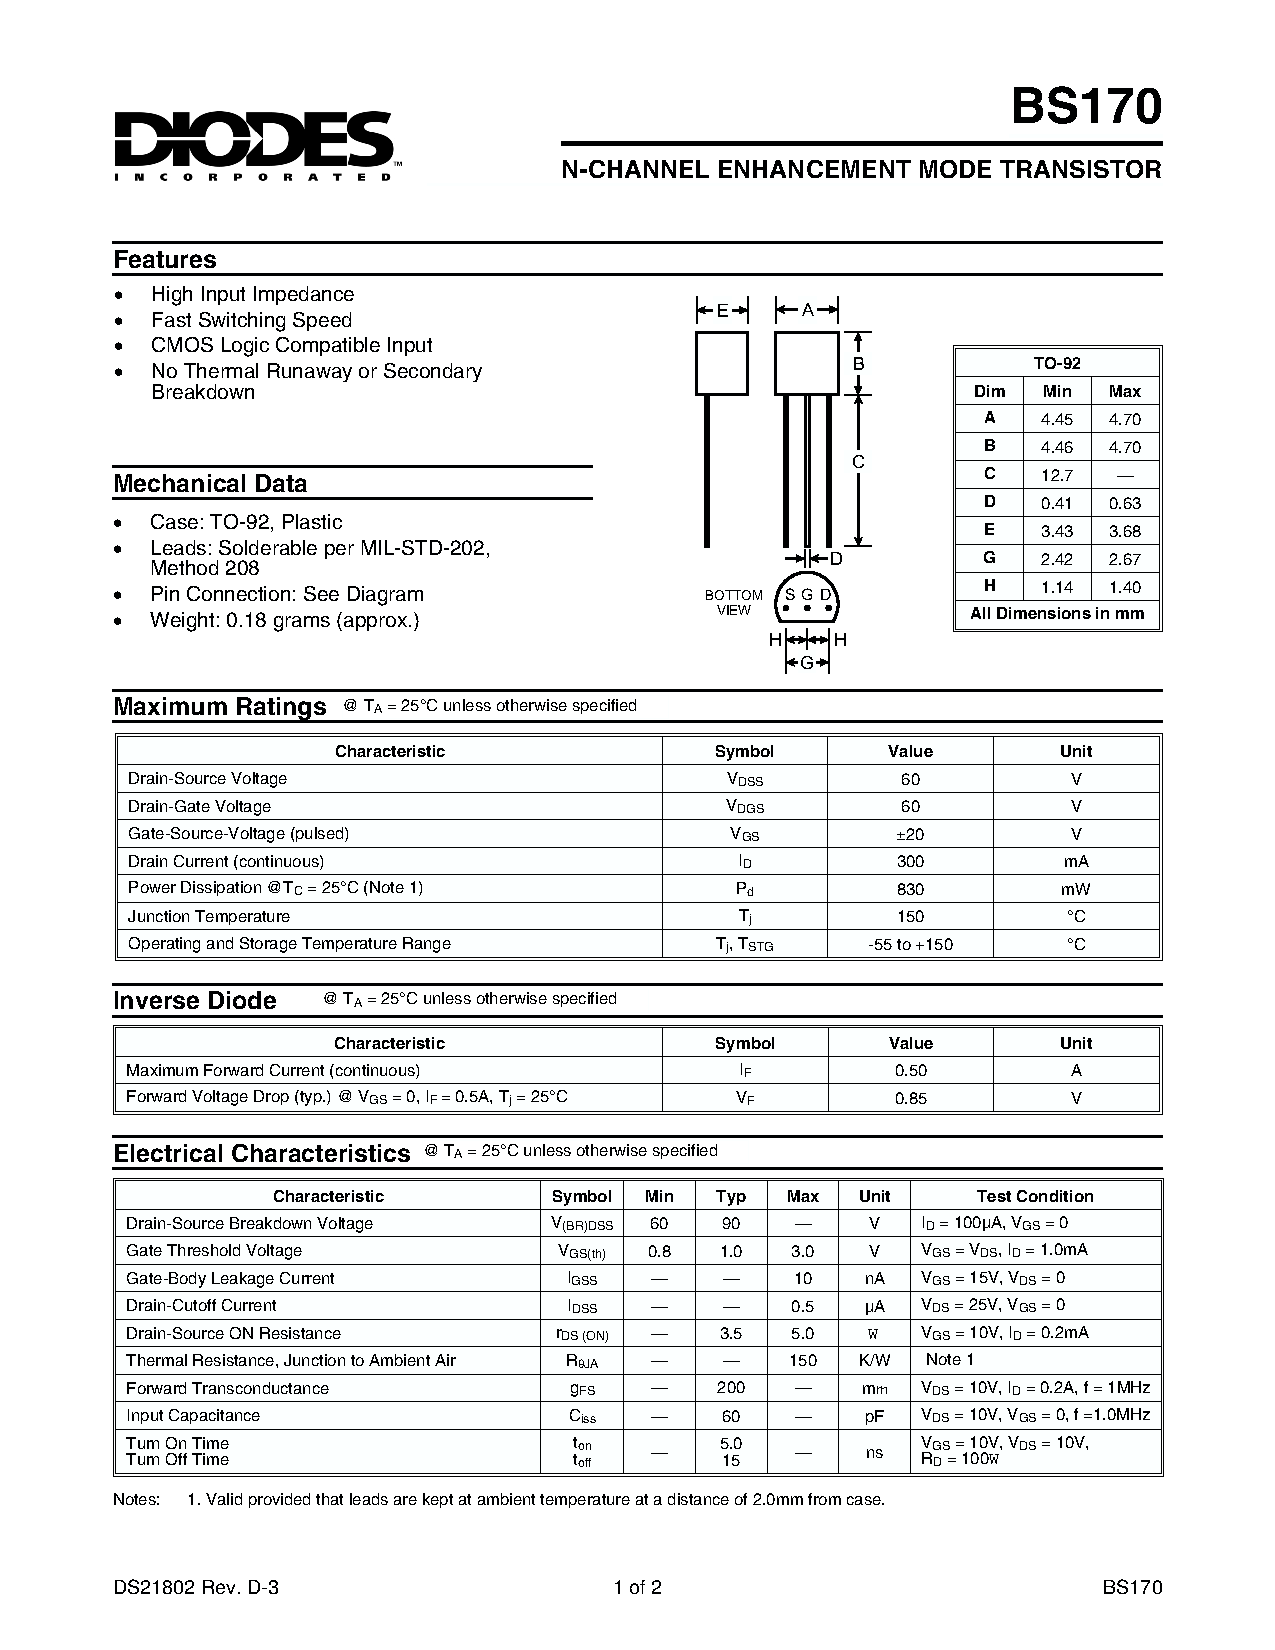
\includepdf[pages={1-2},scale=0.9,pagecommand={\pagestyle{plain}}]{Documentation_BS170.pdf}

\end{document}
